\documentclass[conference]{IEEEtran}
\usepackage{graphicx}
\usepackage{amsmath}
\usepackage{placeins}
\usepackage{xparse}
\usepackage{caption}


\graphicspath{ {images/} }
\providecommand{\norm}[1]{\lVert#1\rVert}
\renewcommand\arraystretch{1.5}
\captionsetup[figure]{labelfont={bf},  font={small}}
\captionsetup[table]{labelfont={bf}, font={small}}
\def\tablename{Table}
\pagestyle{plain}


\begin{document}
    \section{Orientacion}

    \subsection{Cuaternión}
        Los cuaterniones son números hipercomplejos, siend una extension de los números reales, similar a la de los números complejos convencionales.
        
        Mientras que los números complejos son una extensión de los reales por la adición de la unidad imaginaria \textbf{$ i $}, tal que \textbf{$ i^2 = -1 $}
        , los cuaterniones son una extensión generada de manera análoga, añadiendo las unidades imaginarias: $i, j$ y $ k $ a los números reales 
        y tal que $ i^2 = j^2 = k^2 = ijk = -1$.

            \begin{table}[htp]
                \centering
                    \begin{tabular}{|c|c|c|c|c|}
                        \hline
                        \textbf{x} & 1 & i  & j  & k \\ \hline
                             1 & 1 & i  & j  & k \\ \hline
                             i & i & -1 & k  & -j \\ \hline
                             j & j & -k & -1 & i \\ \hline
                             k & k & j  & -i & -1 \\ 
                        \hline
                    \end{tabular}
                \caption{Tabla de Cayley}
                \label{table: Cayley}
            \end{table}

        La tabla \ref{table: Cayley} naos describe como es la operacion de las componentes entre si para un cuaternión.

        Un cuaternión tiene la siguiente forma y estructura:
        $$ q = [a, \hspace{1mm} b, \hspace{1mm} c, \hspace{1mm} d]$$
        $$ q = a + bi +cj + dk $$

        Donde a, b, c y d son números reales unívocamente determinados por cada cuaternión y 
        1, $ i, j $ y $ k $, son entonces las componentes "base" de un cuaternión.

        Con los cuaterniones podemos realizar las 4 operaciones basicas con sus respectivas propiedades, estas operaciones son
        suma, resta, producto y cociente, solo hay que tener en cuenta que el producto no es conmitativo, el orden de los operandos
        si afecta.
        $$  q_{a+b} = q_a + q_b $$
        $$  q_{a-b} = q_a - q_b $$
        $$  q_{a \otimes b} = q_a \otimes q_b $$
        $$  q_{a \otimes b} \neq q_{b \otimes a}  $$
        $$  \frac{q_a}{q_b} = \frac{q_{ab}}{(\norm{q_b})^2} $$

    \subsection{Filtro de Mahony}
    Es un filtro del tipo complementario, su principal objetivo es el mejorar la estimación de la orientación, aplicando un filtro pasa bajas a las estimaciones obtenidas del acelerómetro y magnetómetro, paralelamente aplicando un filtro pasa altas a las estimaciones obtenidas del giroscopio, para al final fusionar estas dos estimaciones y así obtener una estimación más precisa de la orientación. 
    
    Este filtro tiene dos parametros modificables, los cuales son \textbf{\textit{Kp}} y \textbf{\textit{Ki}}, los cuales son el control integral y el control proporcional respectivamente. De igual forma que con otro tipo de filtros de la misma índole, este se basa en una representación en forma de cuaterniones.
    \begin{figure}[htp]
        \centering
             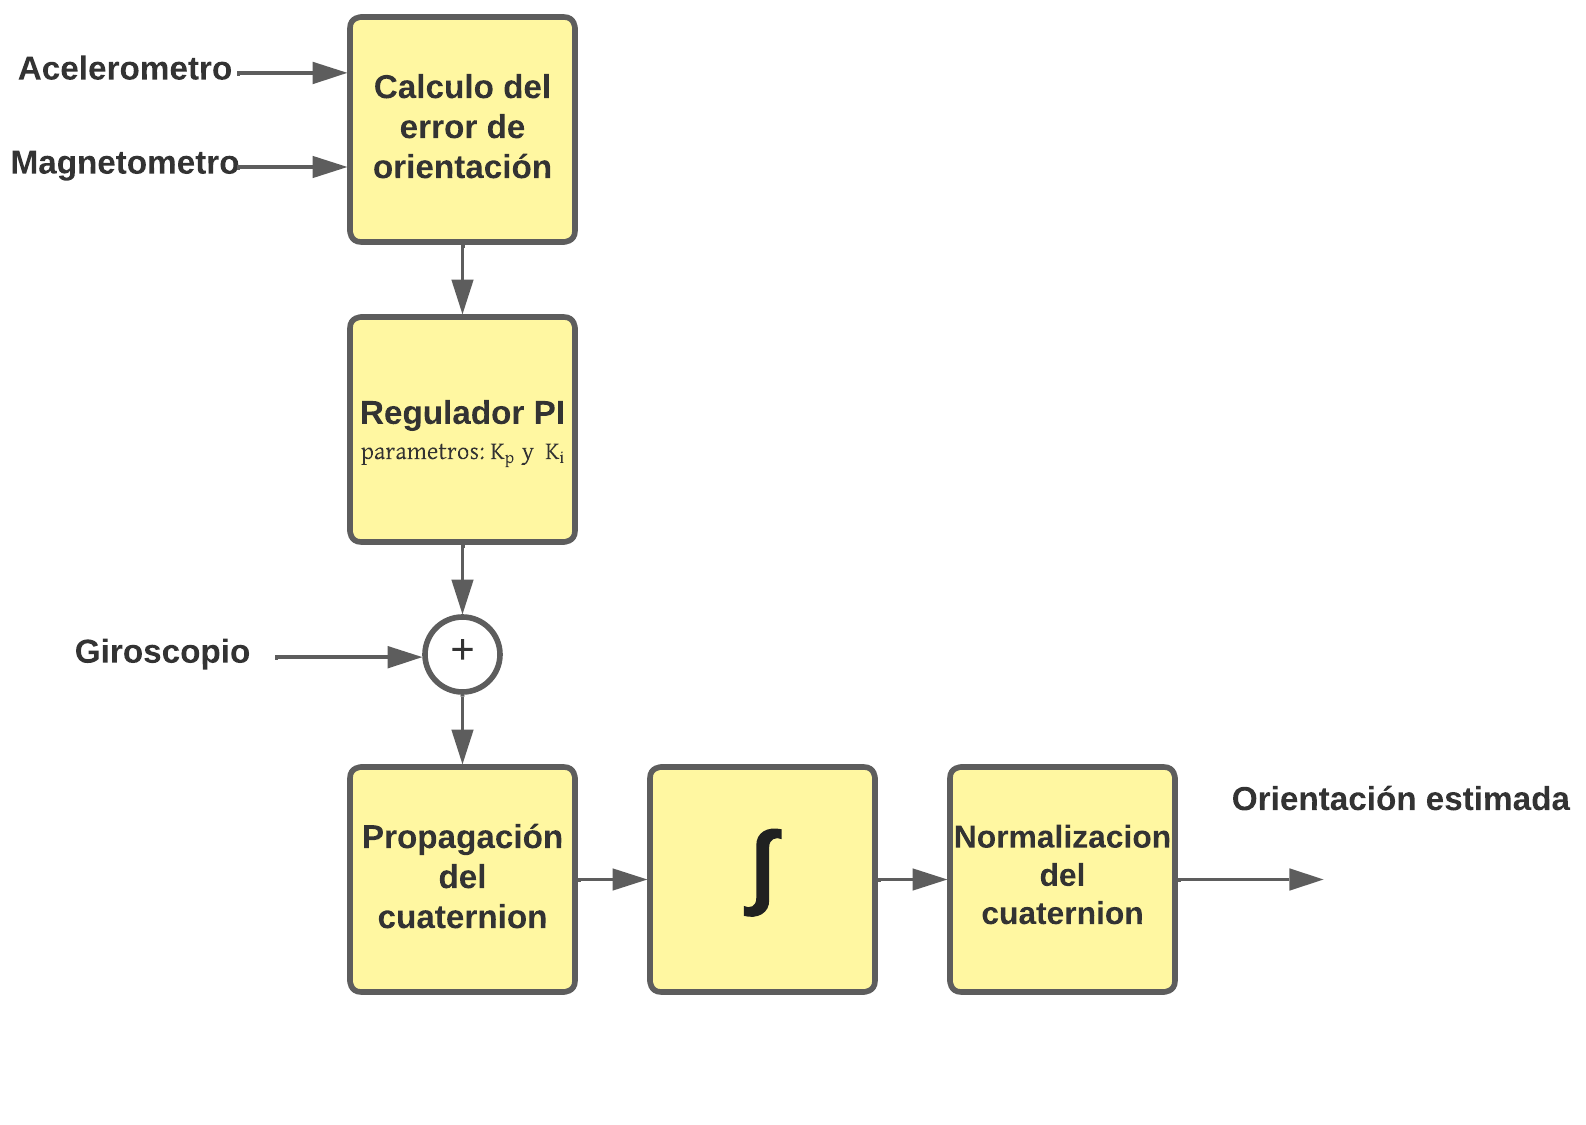
\includegraphics[width=\columnwidth]{mahony_block_diagram_vertical.png}
              \caption{Diagrama a bloques del filtro de Mahony}
    \end{figure}
    \FloatBarrier 


    \textbf{Implementación}

    Para este proyecto, el filtro se aplicó para obtener una mejor estimación sobre la orientación del lactante, el filtro fue implementado de la siguiente manera:

    \begin{enumerate}
        \item Se normalizan los vectores con las estimaciones del acelerómetro y magnetómetro obtenidas en la iteración actual:
        \begin{equation}
             \vec{a_k} = [a_{x,k}, a_{y,k}, a_{z,k}]  
        \end{equation}

        \begin{equation}
            \hat{a_k} = \frac{\vec{a_k}}{\norm{\vec{a_k}}}  
        \end{equation}

        \begin{equation}
            \vec{m_k} = [m_{x,k}, m_{y,k}, m_{z,k}] 
        \end{equation}

        \begin{equation}
            \hat{m_k} = \frac{\vec{m_k}}{\norm{\vec{m_k}}} 
        \end{equation}
            
        
        \item Se establece la referencia a la dirección del campo magnético terrestre, utilizando las estimaciones del magnetómetro y los valores del cuaternión calculado en la iteración anterior:
        
        \begin{equation}
            \resizebox{0.84\hsize}{!}{$
            \vec{h} = 
                \begin{bmatrix}
                    2[(m_x,k)(\frac{1}{2} - q^2_3 - q^2_4 ) + (m_y,k)(q_2q_3 - q_1q_4) + (m_z,k)(q_2q_3 + q_1q_4)] \\
                    2[(m_x,k)(q_2q_3 + q_1q_4) + (m_y,k)(\frac{1}{2} - q^2_2 - q^2_4 ) + (m_z,k)(q_3q_4 - q_1q_2)] \\
                    0 
                \end{bmatrix} 
            $}    
        \end{equation}
        
        
        \begin{equation}
        \resizebox{0.84\hsize}{!}{$
            \vec{b} = 
                \begin{bmatrix}
                    \sqrt[2]{(h_x)^2+(h_y)^2}  \\
                    0 \\
                    2[(m_x,k)(q_2q_4 - q_1q_3) + (m_y,k)(q_3q_4 - q_1q_2) + (m_z,k)(\frac{1}{2} - q^2_2 - q^2_3 )] 
                \end{bmatrix} 
            $}
        \end{equation}
            
        \item Se estima la dirección del campo gravitacional \textbf{\textit{$\vec{v}$}} y campo magnético \textbf{\textit{$\vec{w}$}} con referencia al IMU, utilizando la referencia calculada en el paso anterior y los valores del cuaternión calculados en la iteración anterior:
        
        \begin{equation}        
            \vec{v} = 
                \begin{bmatrix}
                    2(q_2q_4 - q_1q_3) \\
                    2(q_1q_2 + q_3q_4) \\
                    q^2_1 - q^2_2 - q^2_3 +q^2_4  
                \end{bmatrix} 
        \end{equation}

        \begin{equation}        
            \vec{w} = 
                \begin{bmatrix}
                    2[(b_x)(\frac{1}{2} - q^2_3 - q^2_4) + (b_z)(q_2q_4 - q_1q_3)] \\
                    2[(b_x)(q_2q_3 - q_1q_4) + (b_z)(q_1q_2 + q_3q_4)] \\
                    2[(b_x)(q_1q_3 + q_2q_4) + (b_z)(\frac{1}{2} - q^2_2 - q^2_3)] 
                \end{bmatrix} 
        \end{equation}

        \item Se calcula el error $\vec{e}$, como la suma de los productos cruz entre las direcciones de referencia y las medidas, tanto del campo gravitatorio como del magnético:
        
        \begin{equation}
            \vec{e} = (\vec{a_k} \times \vec{v}) + (\vec{m_k} \times \vec{w}) 
        \end{equation}
            
        \begin{equation}
            \vec{e} = 
                \begin{bmatrix}
                    (a_{y,k}v_z - a_{z,k}v_y) + (m_{y,k}w_z - m_{x,w}v_y) \\
                    (a_{z,k}v_x - a_{x,k}v_z) + (m_{z,k}w_x - m_{z,w}v_z) \\
                    (a_{x,k}v_y - a_{y,k}v_x) + (m_{x,k}w_y - m_{y,w}v_x) \\
                \end{bmatrix} 
        \end{equation}
            
        \item Se calcula el error de la iteración actual con el valor de error calculado en el paso anterior multiplicado por un diferencial del tiempo más lo ya acumulado de iteraciones pasadas:
 
        \begin{equation}
                E_k = E_{k-1} + e\Delta t
        \end{equation}

        \item Se calcula el vector de velocidad angular corregido con las mediciones recabadas por el giroscopio, el error calculado en los dos pasos anteriores y los valores de las ganancias tanto proporcional \textbf{\textit{Kp}} como integral \textbf{\textit{Ki}}:
        
        \begin{equation}
            \vec{w_k} = \vec{w_k}_{-1} + K_pe +K_iE_k 
        \end{equation}
            
        \item El vector de velocidad angular corregido es utilizado en conjunto con el cuaternión de la iteración anterior para calcular la tasa de cambio o derivada del cuaternión de orientación actual:
        
        \begin{equation}
            \dot{q} = \frac{1}{2}{q_k}_{-1} \otimes \vec{w_k} 
        \end{equation}
        \begin{equation}
            \dot{q} = \frac{1}{2}[q_1, \hspace{1mm} q_2, \hspace{1mm} q_3, \hspace{1mm} q_4] \otimes [0, \hspace{1mm} w_{x,k}, \hspace{1mm} w_{y,k}, \hspace{1mm} w_{z,k}] 
        \end{equation}

        Donde el caracter $ \otimes $  indica una multiplicacion entre cuaterniones, quedando de la siguiente forma:
        \begin{equation}
            \dot{q} = 
                \begin{bmatrix}
                    \frac{1}{2}(-q_2w_{x,k} - q_3w_{y,k} - q_4w_{z,k}) \\
                    \frac{1}{2}( q_1w_{x,k} + q_3w_{z,k} - q_4w_{y,k}) \\
                    \frac{1}{2}( q_1w_{y,k} - q_2w_{z,k} + q_4w_{x,k}) \\
                    \frac{1}{2}( q_1w_{z,k} + q_2w_{y,k} - q_3w_{x,k}) \\
                \end{bmatrix} 
        \end{equation}    

        \item El resultado del paso anterior se integra de la siguiente manera para así obtener el cuaternión de orientación de la iteración actual:
        
        \begin{equation}
            q_k = q_{k-1} + \dot{q} \Delta t 
        \end{equation}
    
        \item Finalmente, se normaliza (este se normaliza como si se tratase de un vector) y obtenemos la estimacion de la orientacion en terminos de cuaterniones:
        \begin{equation}
            \hat{q_k} = \frac{q_k}{\norm{q_k}} 
        \end{equation}        
            
        \begin{equation} \label{eq:18}
            \hat{q_k} = \frac{q_1, \hspace{1mm} q_2, \hspace{1mm} q_3, \hspace{1mm} q_4}{\sqrt[2]{(q_1)^2 + (q_2)^2 + (q_3)^2 + (q_4)^2}} 
        \end{equation}
            
    \end{enumerate}

    \subsection{Angulos de Tait-Bryan}

    Además de la representación por cuaterniones, se tiene como alternativa los ángulos de Tait-Bryan para poder representar la orientación, mediante funciones
    trigonometricas y utilizando el resultado entregado por la ecuación \ref{eq:18} se puede obtener la inclinacion en los ejes x, y, z, los cuales se conocen 
    como \textbf{Roll ($ \phi $)}, \textbf{Pitch ($ \theta  $)}, y \textbf{Yaw ($ \psi  $)} respectivamente.

    \begin{figure}[htp!]
        \centering
             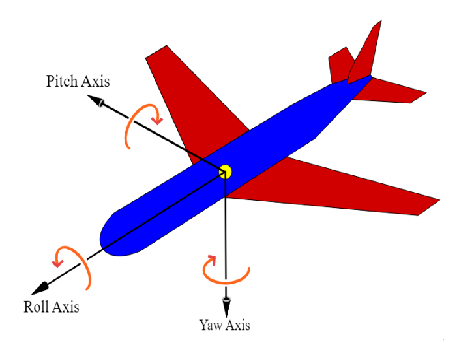
\includegraphics[width=\columnwidth]{tait-bryan_axis_representation.png}
              \caption{Representacion de la orientación de un objeto mediante los ángulos de Tait-Bryan}
    \end{figure}
    \FloatBarrier 

    Las formulas para calcular estos ángulos son las siguientes:

    \begin{equation}
        \begin{bmatrix}
            \phi \\ \theta \\ \psi 
        \end{bmatrix} =
            \begin{bmatrix}
                \arctan \left (\frac{q_1q_2 + q_3q_4}{\frac{1}{2}-(q^2_2+q^2_3)} \right ) \\
                \arcsin  (2(q_1q_3-q_2q_4)) \\
                \arctan \left (\frac{q_1q_4 + q_2q_3}{\frac{1}{2}-(q^2_3+q^2_4)} \right ) \\
            \end{bmatrix}
    \end{equation}

    Para el presente proyecto, se hicieron pruebas con ambos tipos de representación para la orientación, 
    donde se opto por la del cuaternión, debido a que tiene menos limitantes que la de angulos de Tait-Bryan.
\end{document}
